\documentclass[10pt,a4paper,landscape]{article}
\usepackage[utf8]{inputenc}
\usepackage{amsmath}
\usepackage{amsfonts}
\usepackage{amssymb}
\usepackage{graphicx}
\usepackage[left=0.5cm,right=0.5cm,top=0.5cm,bottom=0.5cm]{geometry}
% \usepackage{tikz}
% \usepackage{subfiles}
\graphicspath{{../Figures/}} % Directory in which figures are stored
\begin{document}
\centering
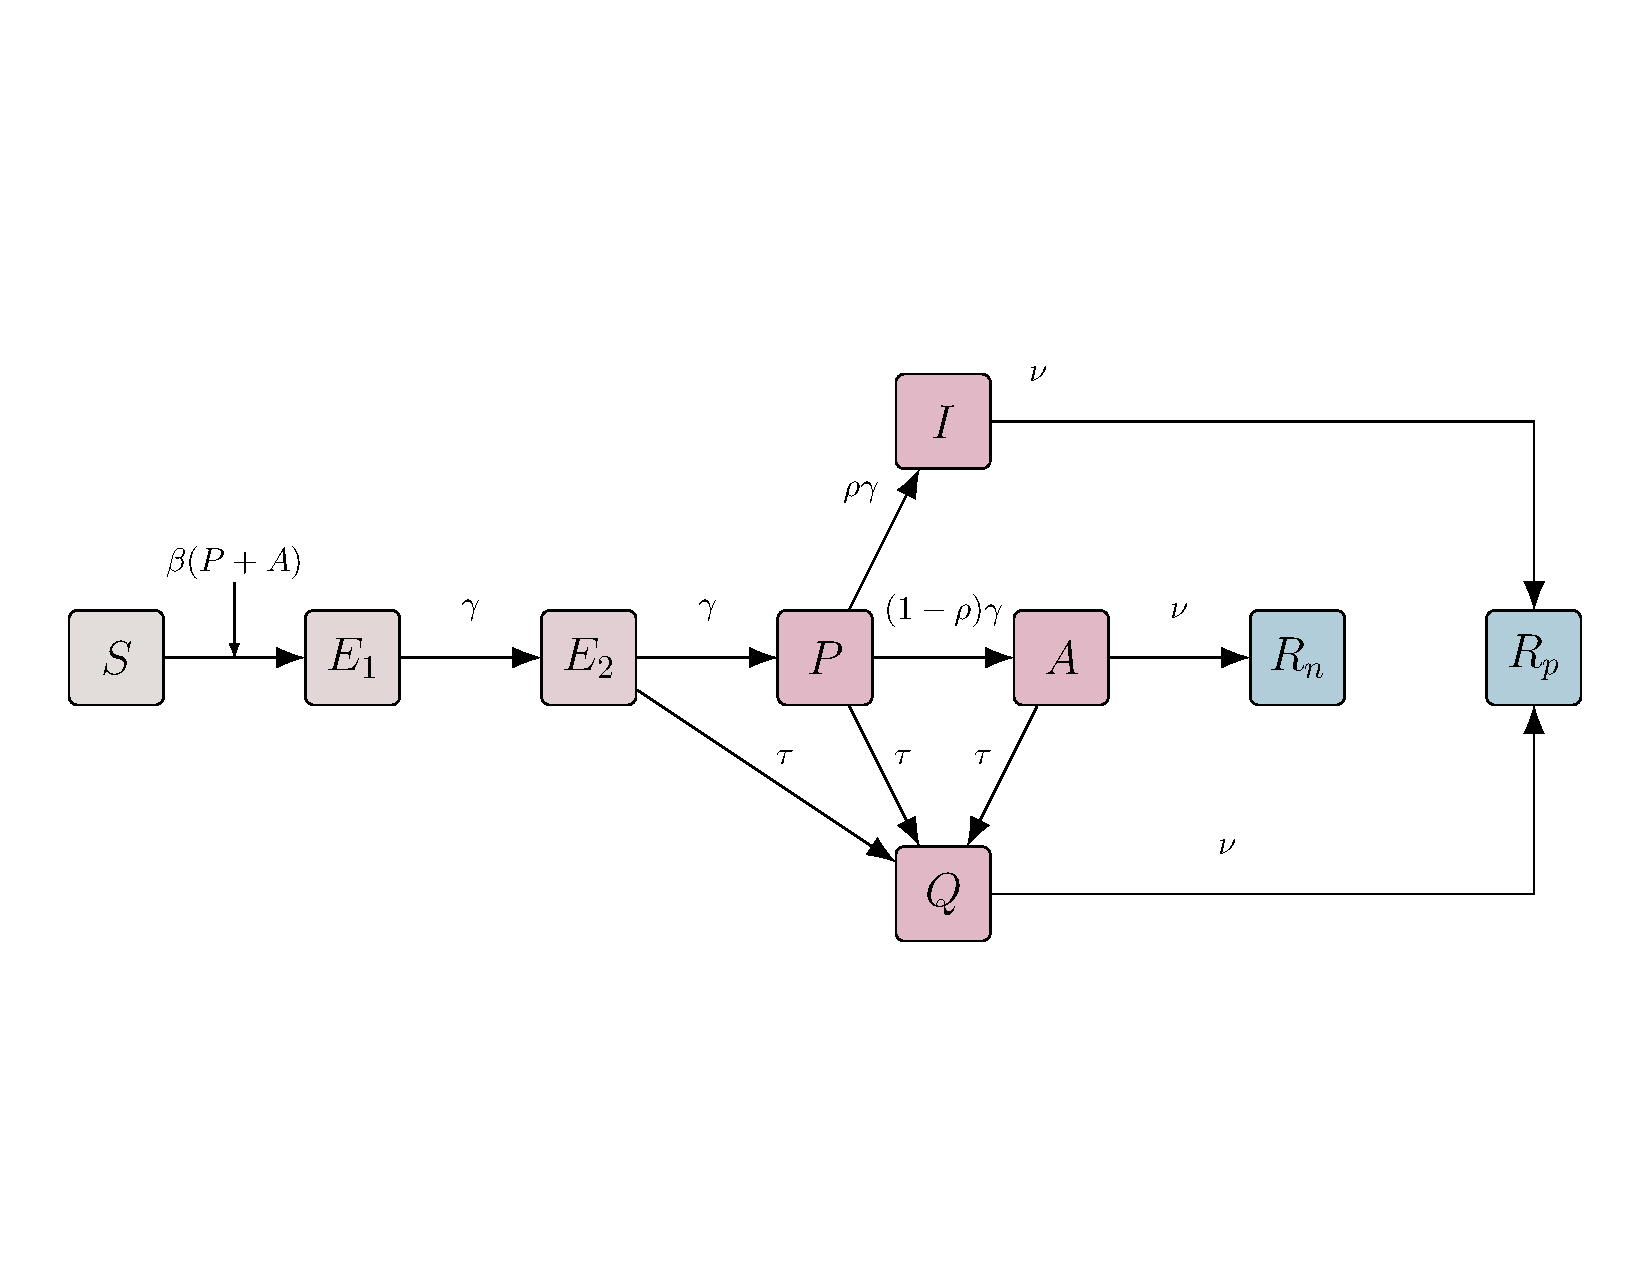
\includegraphics[width=0.9\linewidth]{../Descriptions/TestIntensityFigure.pdf}

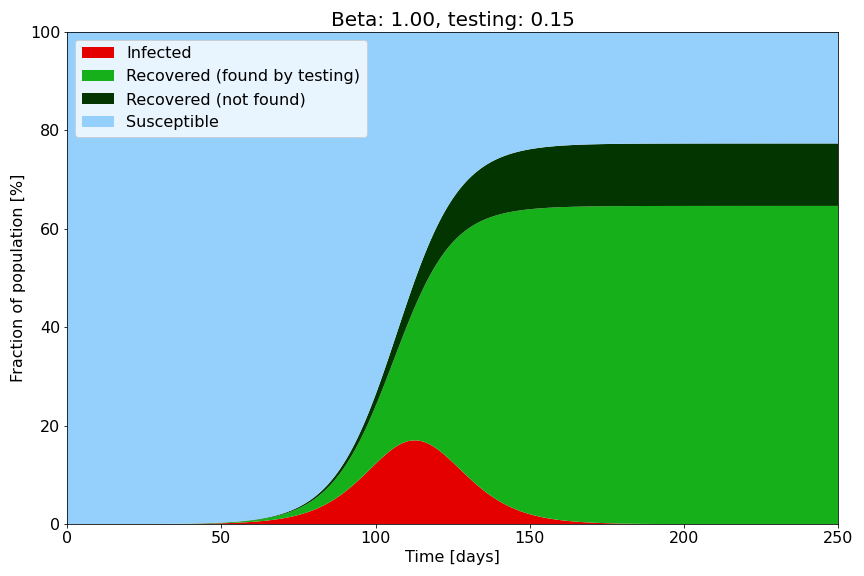
\includegraphics[width=0.98\linewidth]{TestIntensity_ExampleStacked.png}

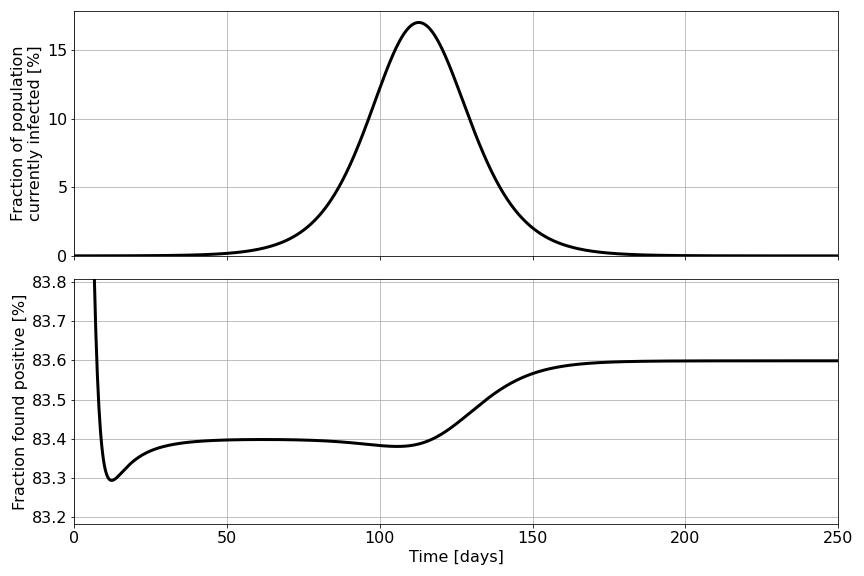
\includegraphics[width=0.98\linewidth]{TestIntensity_ExampleTestRatio.png}

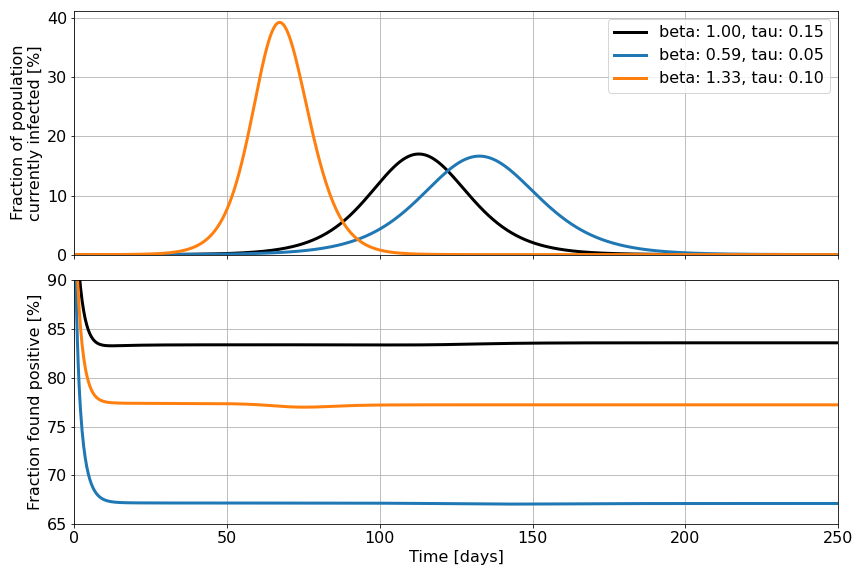
\includegraphics[width=0.98\linewidth]{TestIntensity_ExampleTestRatioMultiple.png}

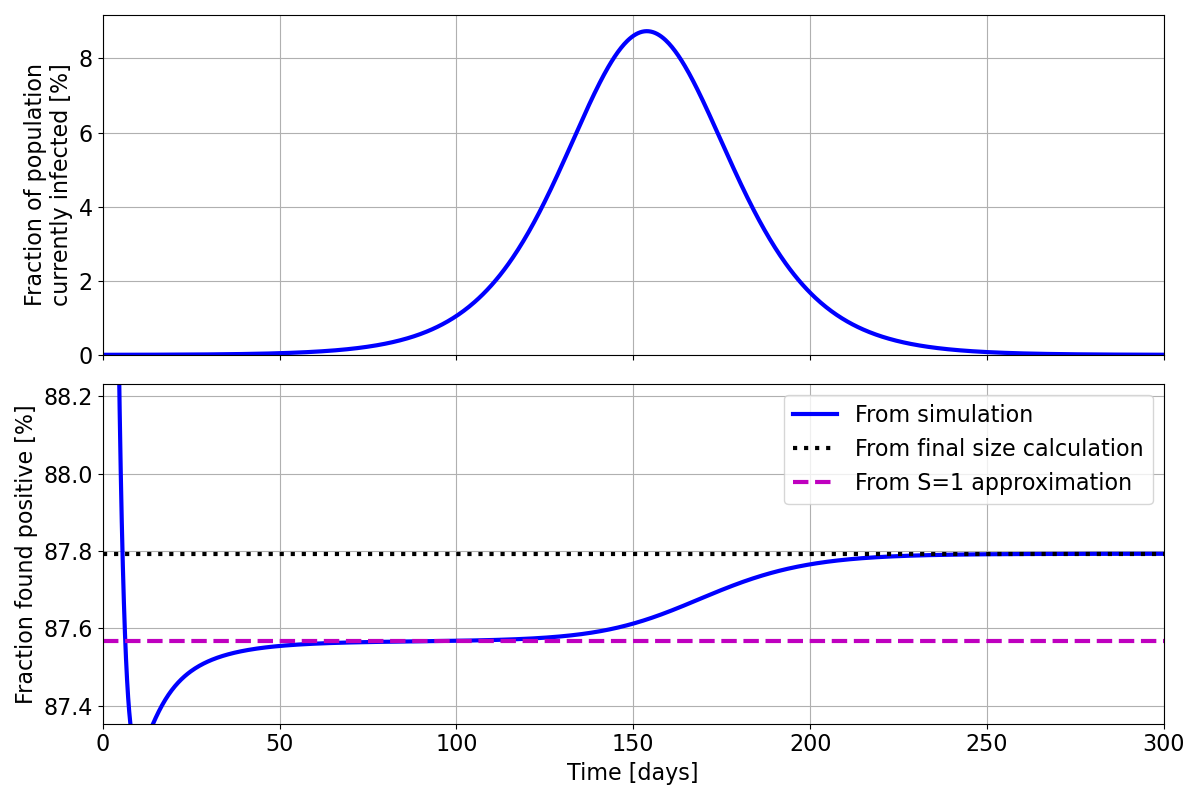
\includegraphics[width=0.98\linewidth]{TestIntensity_ExampleTestRatioWithLevels.png}

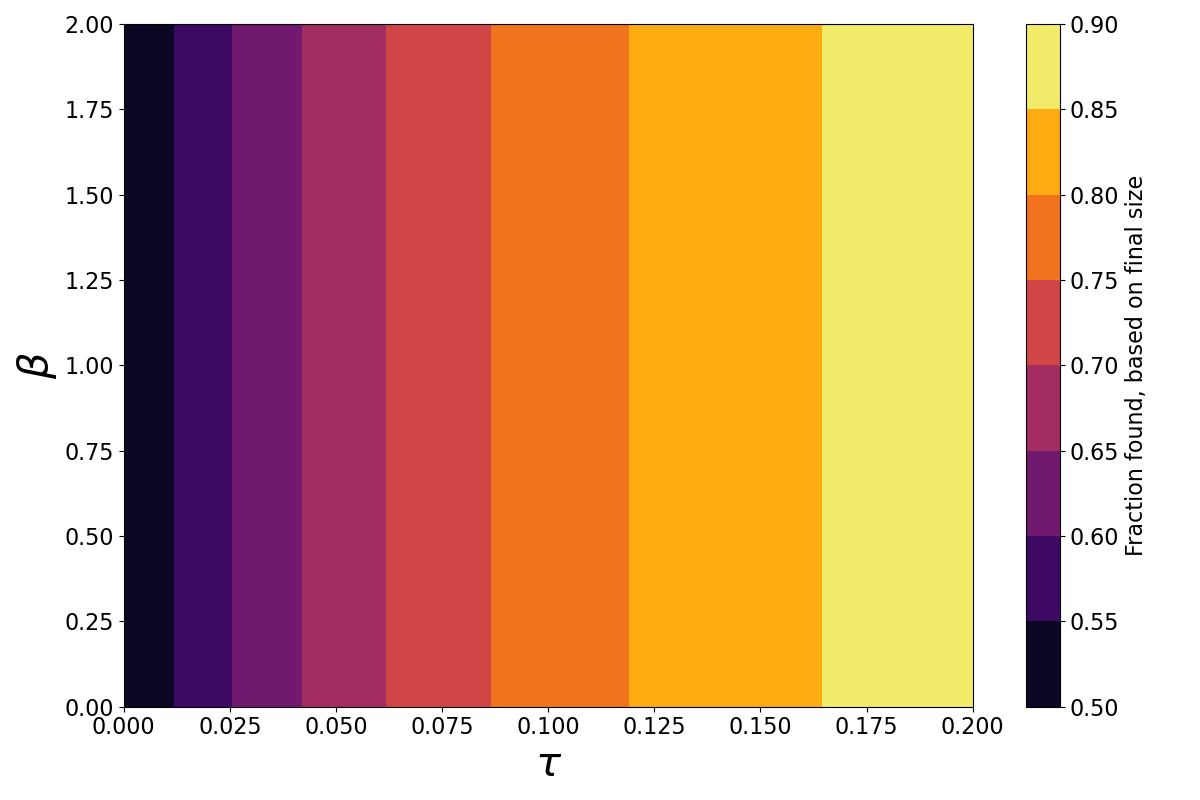
\includegraphics[width=0.98\linewidth]{TestIntensity_RatioFinal.png}

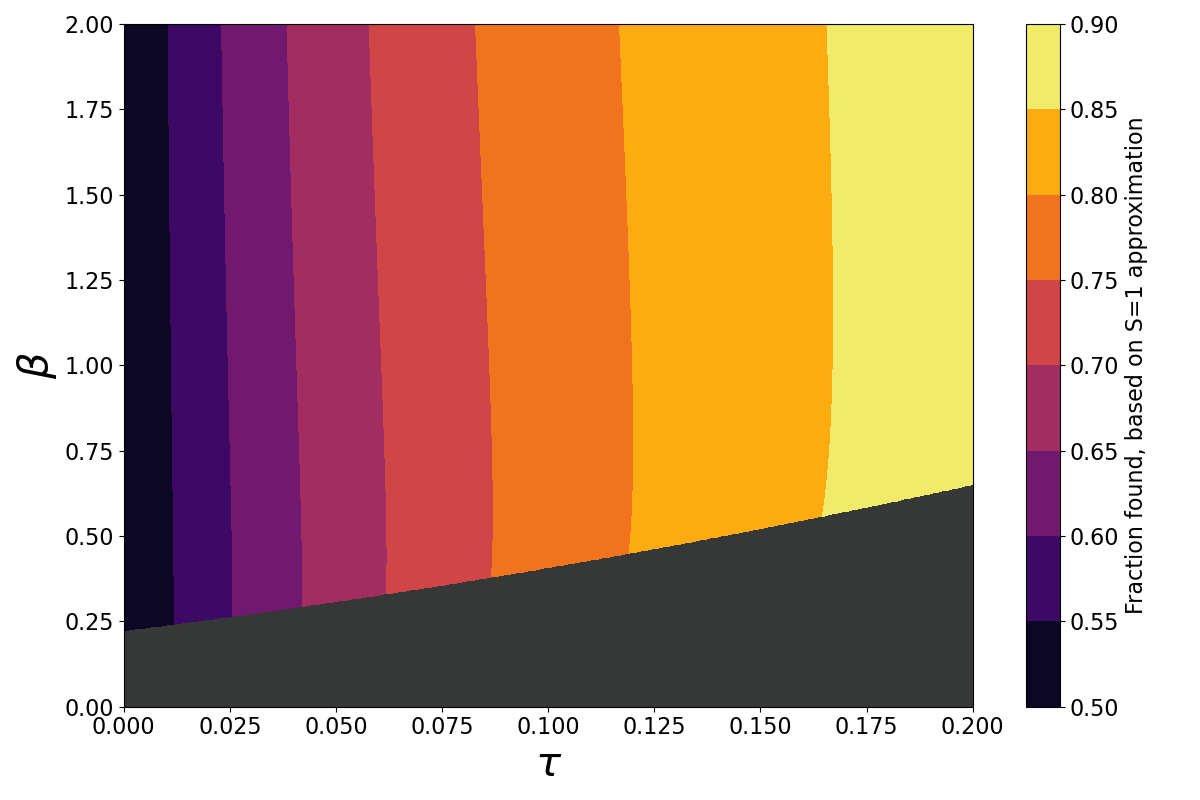
\includegraphics[width=0.98\linewidth]{TestIntensity_RatioBefore.png}

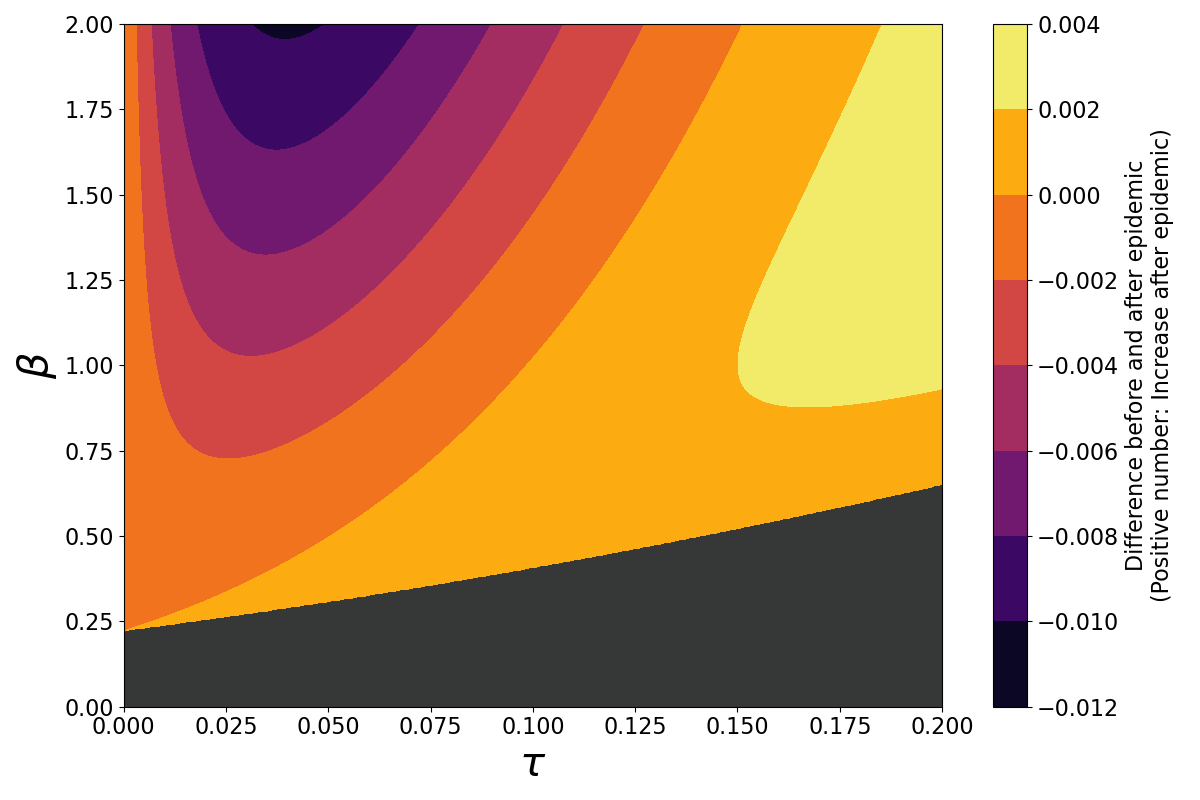
\includegraphics[width=0.98\linewidth]{TestIntensity_RatioDifference.png}

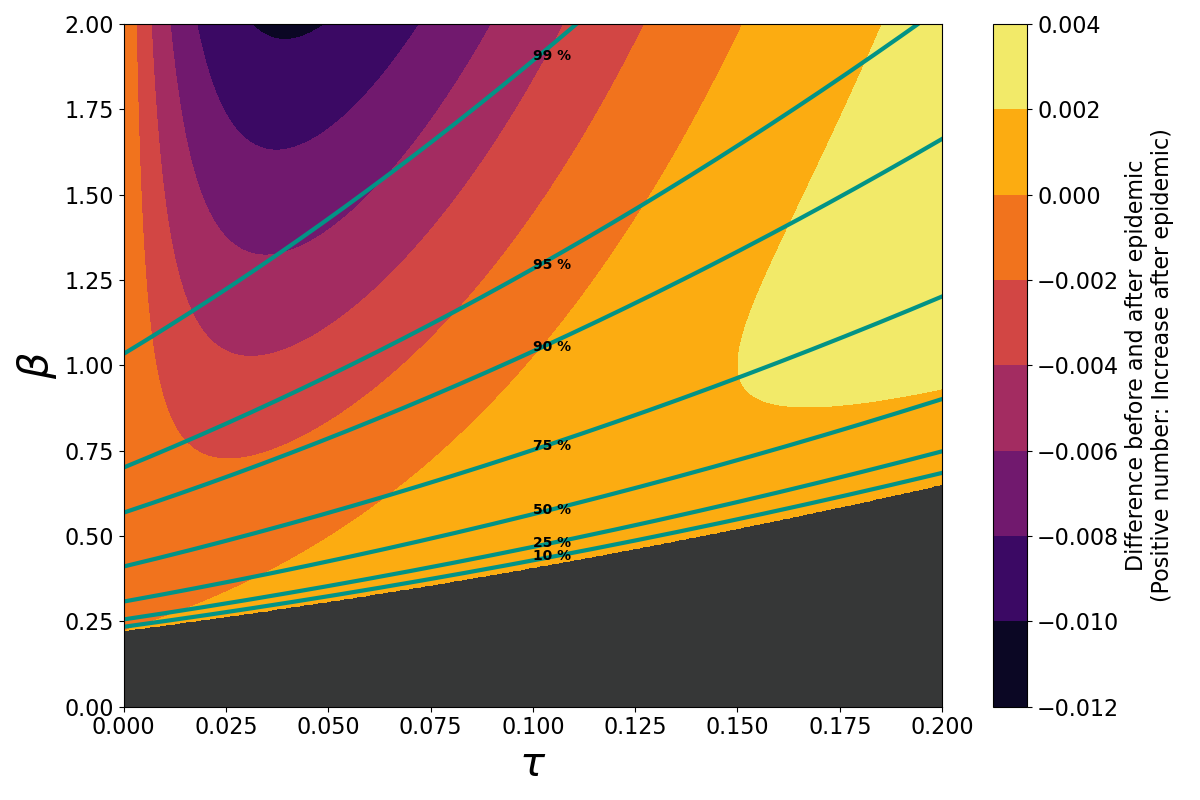
\includegraphics[width=0.98\linewidth]{TestIntensity_RatioDifferenceLines.png}

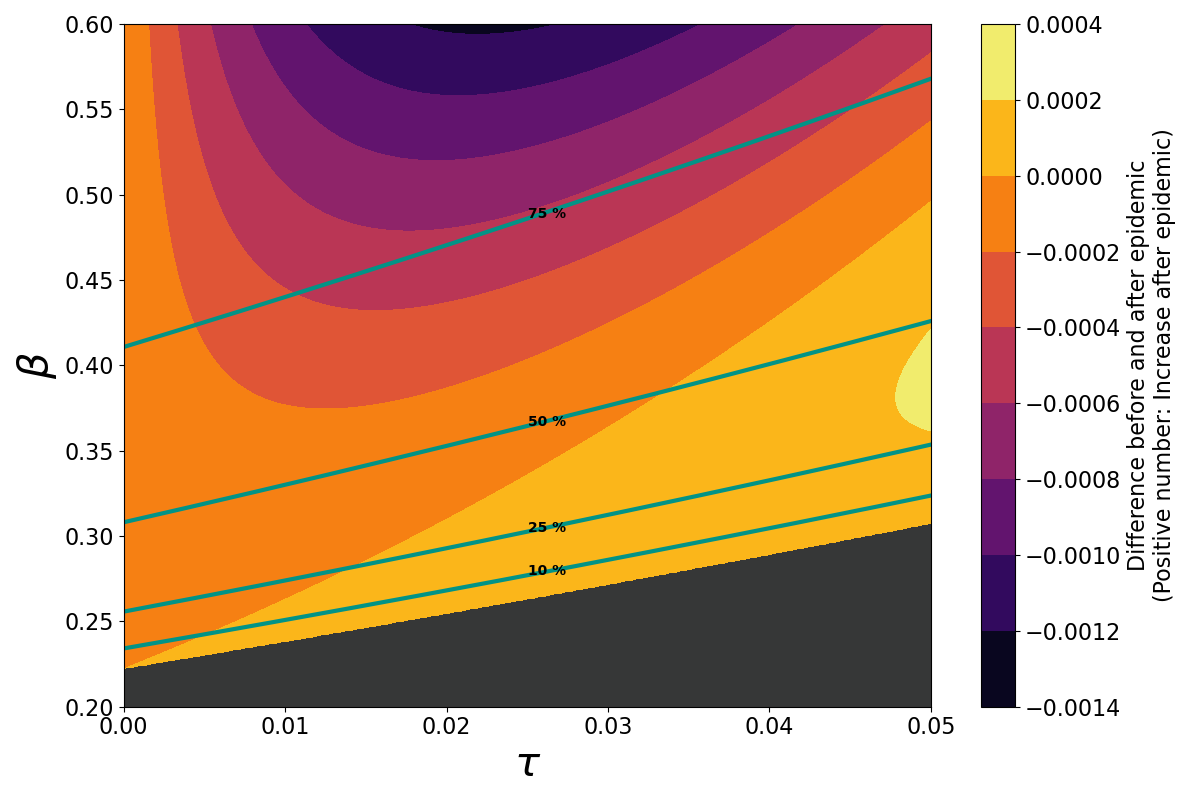
\includegraphics[width=0.98\linewidth]{TestIntensity_RatioDifferenceLines_Zoom.png}

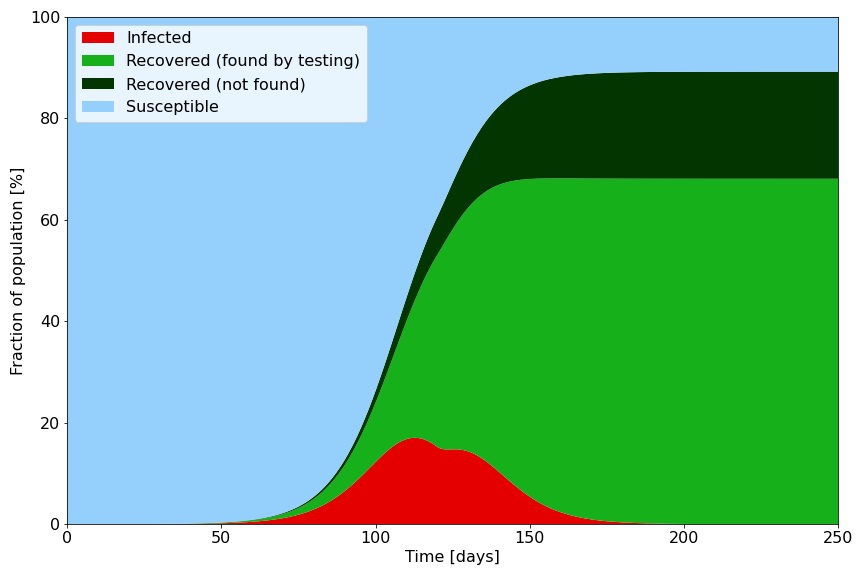
\includegraphics[width=0.98\linewidth]{TestIntensity_ExampleStackedChange.png}

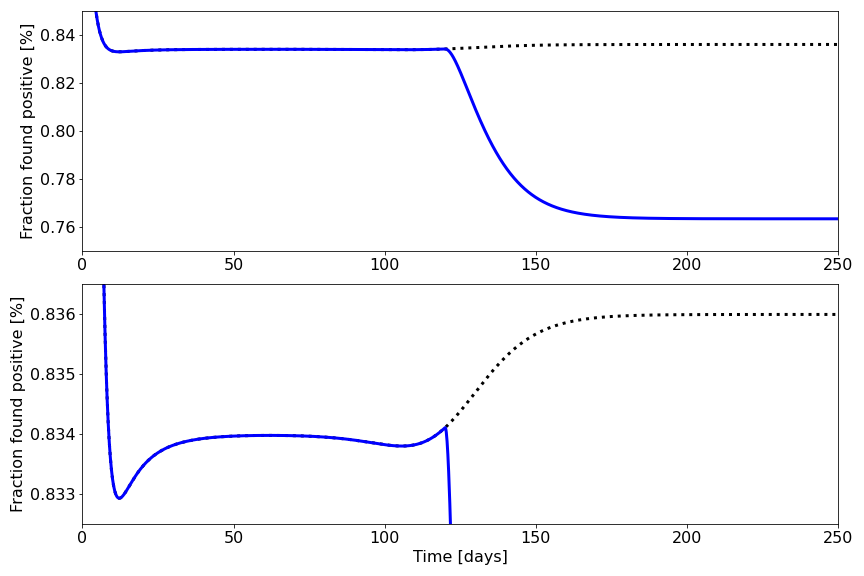
\includegraphics[width=0.98\linewidth]{TestIntensity_ExampleChangeRatio.png}


\end{document}

% \documentclass[11pt,usenames,dvipsnames]{beamer}
% \setbeamercolor{structure}{fg=OliveGreen!90!black,bg=gray!5!white}
% \setbeamercolor{palette primary}{fg=OliveGreen,bg=gray!80!white}
% \setbeamercolor{palette secondary}{fg=OliveGreen!70!black,bg=gray!15!white}
% \setbeamercolor{palette tertiary}{bg=OliveGreen!80!black,fg=gray!10!white}
% \setbeamercolor{palette quaternary}{fg=OliveGreen,bg=gray!5!white}
% \setbeamercolor{section in sidebar shaded}{fg=gray!10!black}
% \setbeamercolor{palette sidebar primary}{fg=black,bg=OliveGreen!10!white}
% \setbeamercolor{palette sidebar secondary}{fg=black,bg=OliveGreen!5!white}
% \setbeamercolor{palette sidebar tertiary}{fg=black,bg=OliveGreen!20!white}
% \setbeamercolor{palette sidebar quaternary}{fg=black,bg=OliveGreen!20!white}
% \setbeamercolor{structure}{fg=OliveGreen!60!black,bg=gray!5!white}
% \setbeamercolor{palette primary}{fg=OliveGreen,bg=gray!80!white}
% \setbeamercolor{palette secondary}{fg=OliveGreen!70!black,bg=gray!15!white}
% \setbeamercolor{palette tertiary}{bg=OliveGreen!80!black,fg=gray!10!white}
% \setbeamercolor{palette quaternary}{fg=OliveGreen,bg=gray!5!white}
% \setbeamercolor{section in sidebar shaded}{fg=gray!10!black}
% \setbeamercolor{palette sidebar primary}{fg=black,bg=OliveGreen!10!white}
% \setbeamercolor{palette sidebar secondary}{fg=black,bg=OliveGreen!5!white}
% \setbeamercolor{palette sidebar tertiary}{fg=black,bg=OliveGreen!20!white}
% \setbeamercolor{palette sidebar quaternary}{fg=black,bg=OliveGreen!20!white}
% \usetheme{Goettingen}
% %\usetheme{Darmstadt}
% %\usecolortheme{seahorse}
% %\usetheme{Goettingen}
% %\usecolortheme{rose}
% \usepackage[utf8]{inputenc}
% \usepackage{amsmath}
% \usepackage{amsfonts}
% \usepackage{amssymb}
% \usepackage{ulem}
% \usepackage{subcaption}
% \usepackage{hyperref}
% \usepackage{todonotes}
% \usepackage{graphicx}
% %\usepackage{animate}
% \usepackage{natbib}
% %\bibliographystyle{agsm}
% \bibliographystyle{humannat}

% % Remove the beamer-buttons
% \setbeamertemplate{navigation symbols}{}

% %\usepackage{tikz}
% %\usetikzlibrary{calc}
% %\usetikzlibrary{arrows.meta}
% %\usetikzlibrary{patterns}
% %\tikzset{
% %niche/.pic = {
% %           \begin{scope}[scale=#1,every node/.style={scale=0.8*#1}]
% %			\draw[fill=gray] (0.5,0) arc(0:-180:0.5) -- (-.5,-1) -- (0.5,-1) --(0.5,0);
% %            \end{scope}
% %			}			
% %}
% %\definecolor{cellColor}{cmyk}{0.33,0.10,0,0}
% %\definecolor{cellColorDiff}{cmyk}{0.66,0.33,0.66,0}
% %\definecolor{cellColor2}{cmyk}{0,0.33,0.33,0}
% %\definecolor{cellColor2Diff}{cmyk}{0.33,0.66,0.33,0}
% %\definecolor{lightgrey}{cmyk}{0,0,0,0.25}
% %\definecolor{nicheCellColor}{cmyk}{0,0.25,0.25,0.25}
% %

% %\definecolor{cellColor}{cmyk}{0.33,0.10,0,0.13} % Blue
% %\definecolor{cellColor2}{cmyk}{0,0.9,1,0} % Red

% \definecolor{cellColor}{cmyk}{0.33,0.10,0,0}
% \definecolor{cellColorDiff}{cmyk}{0.66,0.33,0.66,0}
% \definecolor{cellColor2}{cmyk}{0,0.33,0.33,0}
% \definecolor{cellColor2Diff}{cmyk}{0.33,0.66,0.33,0}

% %%\setbeamercolor*{palette primary}{fg=darkgreen!60!black,bg=gray!30!white}
% %%\setbeamercolor*{palette secondary}{fg=darkgreen!70!black,bg=gray!15!white}
% %%\setbeamercolor*{palette tertiary}{bg=darkgreen!80!black,fg=gray!10!white}
% %%\setbeamercolor*{palette quaternary}{fg=darkgreen,bg=gray!5!white}
% %
% %\newcommand{\biblio}{\bibliography{C:/Users/rakrpe/Documents/MendeleyBibTeX/NicheModelling} }
% %
% \graphicspath{{figures/}} % Directory in which figures are stored
% \author{Rasmus Kristoffer Pedersen }
% \institute{IMFUFA, Department of Science and Environment \\ Roskilde University, Denmark}
% %\date{Stem Cell Modelling Day \\ September 18$^{th}$, 2019}
% %\date{The First Nordic Biomathematics Days, Helsinki \\ October 22$^{th}$, 2019}
% \date{November 20$^{th}$, 2020}
% \titlegraphic{\includegraphics[scale=0.3]{RegionSjaelland.png} \hspace{10pt} \includegraphics[scale=0.5]{RUCLogo.png}}

% \title[MM of MPNs and HSC]{``Mathematical Modelling of Myeloproliferative Neoplasms and Hematopoietic Stem Cells''}
% \subtitle{Ph.D.-defense}
% %\setbeamercovered{transparent} 
% %\setbeamertemplate{navigation symbols}{} 
% %\logo{} 
% %\institute{} 
% %\date{} 
% %\subject{} 
% \addtobeamertemplate{navigation symbols}{}{%
%     \usebeamerfont{footline}%
%     \usebeamercolor[fg]{footline}%
%     \hspace{1em}%
%     \insertframenumber/\inserttotalframenumber
% }